\chapter{Automatisation du processus d'investigation}
\label{Automatisation du processus d'investigation}
\thispagestyle{fancy}
Lorsqu'une error name (partie \ref{Introduction:Expression du besoin:Hiérarchisation des erreurs}) durant le Filtering test, de nombreuses données du robot sont enregistrées dans un fichier journal (que l'on retrouve plus souvent sous le terme anglais de fichier "log".) Une analyse poussée des données contenues dans ce fichier nous permettre de déterminer la root cause (partie \ref{Introduction:Expression du besoin:Hiérarchisation des erreurs}) liée à l'error name. Afin d'automatiser ce processus d'analyse, on s'appuie sur l'utilisation d'algorithmes d'apprentissage automatique.

\section{Architecture High Level du système proposé}
\label{Automatisation du processus d'investigation: Achitecture High Level du système proposé}
On présente l'architecture haut niveau de notre système permettant l'automatisation de la phase d'investigation des erreurs issues du Filtering Test. On réalise également une analyse de chacune des sous partie du système (i.e. exemples pour l'entrainement, exemple à analyser, modèle d'apprentissage, décision).

\subsubsection{Schéma synoptique High Level}
\label{Automatisation du processus d'investigation: Achitecture High Level du système proposé: Schéma synoptique High Level}
Le schéma fonctionnel de la solution que l'on propose est composé de deux couches: une couche "root cause" et la couche "error name".
\begin{description}
	\item [Couche root cause] La couche root cuase gère la detection d'une contient l'ensemble des 
\end{description} 

\begin{figure}[h]
	\centering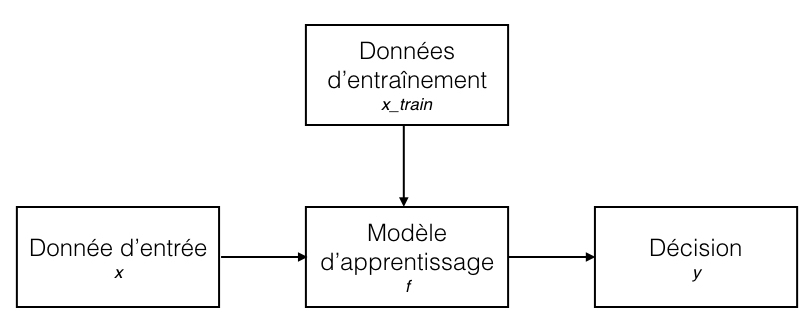
\includegraphics[height=5cm]{images/ML_high_level.jpeg}
	\caption{Schéma synoptique haut niveau de la solution proposée}
	\label{fig:Schéma synoptique haut niveau de la solution proposée}
\end{figure}

\subsubsection{Les exemples pour apprentissage et exemple à analyser}
\label{Automatisation du processus d'investigation: Achitecture High Level du système proposé: Les exemples d'apprentissage}

\subsubsection{Le modèle d'apprentissage}
\label{Automatisation du processus d'investigation: Achitecture High Level du système proposé: Le modèle d'apprentissage}

\subsubsection{La décision}
\label{Automatisation du processus d'investigation: Achitecture High Level du système proposé: La décision}



\section{Solutions techniques testées}
\label{Automatisation du processus d'investigation: Solutions techniques testées}




\section{Solution technique proposée}
\label{Automatisation du processus d'investigation: Solution technique proposée}

